\documentclass{beamer}
\usepackage[english]{babel}

\usepackage{color,hyperref}
\usepackage{amsmath}
\usepackage{amssymb}
\usepackage{amsfonts}
\usepackage{amsopn}
\usepackage{braket}
\usepackage{bbm}
\usepackage{dsfont}
\usepackage{kpfonts}
% \usepackage{mathabx}

\parindent=0cm


% Various new commands that ease typesetting math even further
% \newcommand{\assign}{\ensuremath{\coloneq}}
% \newcommand{\rassign}{\ensuremath{\eqcolon}}
\newcommand{\assign}{\ensuremath{:=}}
\newcommand{\rassign}{\ensuremath{=:}}

\newcommand{\of}[1]{\ensuremath{\left( #1 \right)}}
\newcommand{\ofs}[1]{\ensuremath{\left( #1 \right)}}

\newcommand{\norm}[1]{\ensuremath{\| #1 \|}}

\newcommand{\tmop}[1]{\ensuremath{\operatorname{#1}}}

\newcommand{\id}{\ensuremath{\mathds{1}}}
% \newcommand{\id}{\ensuremath{I}}


\newcommand{\conj}[1]{\ensuremath{\overline{#1}}}

\newcommand{\T}{\ensuremath{{}^{\textnormal{T}}}}
\newcommand{\herm}{\ensuremath{{}^{\textnormal{H}}}}

\newcommand{\ft}[1]{\ensuremath{\mathcal{F}\left(#1\right)}}
\newcommand{\ift}[1]{\ensuremath{\mathcal{F}^{-1}\left(#1\right)}}

\newcommand{\fft}[1]{\ensuremath{\mathtt{FFT}\left(#1\right)}}
\newcommand{\ifft}[1]{\ensuremath{\mathtt{IFFT}\left(#1\right)}}

\newcommand{\dotp}[2]{\ensuremath{\langle #1 , #2 \rangle}}

\newcommand{\bigO}[1]{\ensuremath{\mathcal{O}\left( #1 \right)}}

\newcommand{\mat}[1]{\ensuremath{\mathbf{#1}}}

% multi-indices
\newcommand{\mindex}[1]{\ensuremath{\underline{#1}}}

\newcommand{\laplace}{\ensuremath{\operatorname{\Delta}}}

% EOF

\usepackage{graphicx}
\usepackage{asymptote}
\usepackage[utf8x]{inputenc}

\mode<presentation>
{
  \usetheme{Montpellier}
  \setbeamercovered{transparent}
}

\title[Tunneling dynamics and spawning]{Tunneling dynamics and spawning with adaptive semi-classical wave-packets}
\author[]{V. Gradinaru, G.A. Hagedorn, and A. Joye}
\date{March 10, 2011}

\newcommand{\burl}[1]{\footnotesize{\url{#1}}}

\beamertemplatenavigationsymbolsempty
%-----------------------------------------------------------------------------------------
\begin{document}

\begin{frame}
  \titlepage
\end{frame}


\begin{frame}{Outline}
  \tableofcontents
\end{frame}


\section{Introduction}
\subsection{Schrödinger equation, Potential and Initial Values}


\begin{frame}{Time-dependent Schrödinger equation}
  \begin{equation*} \label{eq:basics_tdse_semi}
    i \varepsilon^2 \frac{\partial}{\partial t} \Ket{\psi} = \underbrace{\left(T+V\right)}_{H} \Ket{\psi}
  \end{equation*}
  where
  \begin{equation*}
    T \assign - \frac{1}{2} \varepsilon^4 \frac{\partial^2}{\partial x^2} \qquad
    V \assign V\ofs{x}
  \end{equation*}
  \begin{itemize}
    \item Time evolution for a state $\Ket{\psi}$
    \item Kinetic operator $T$ and potential $V\left( x \right)$
    \item Semi-classical scaling $\varepsilon^2 \approx 10^{-2}, 10^{-3}, \ldots$
    \item Recover classical mechanics for $\varepsilon \rightarrow 0$
  \end{itemize}
\end{frame}


\begin{frame}{Potential}
  \begin{itemize}
    \item Potential is the one-dimensional Eckart barrier
  \end{itemize}

  \begin{equation*}
    V(x) = \frac{V_0}{\cosh\left(a x\right)}
  \end{equation*}
  \begin{itemize}
    \item $a \approx 2 \cdot 0.52918 \, \text{alu}^{-1}$
    \item $V_0 \approx 100 \, \frac{\text{kJ}}{\text{mol}}$
  \end{itemize}
  \begin{center}
    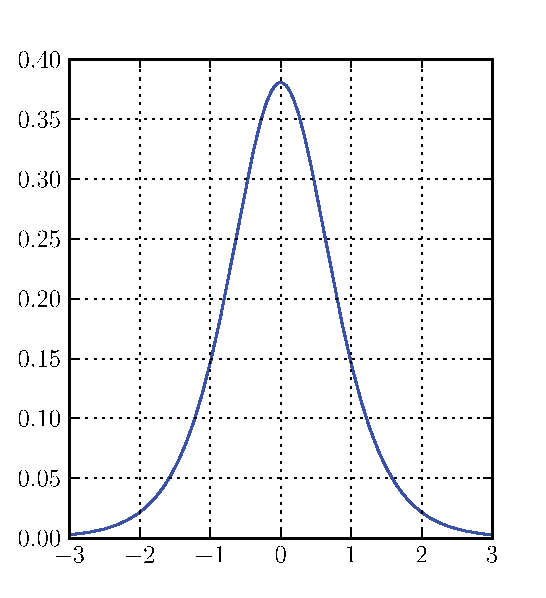
\includegraphics[scale=0.4]{./fig/eckart.pdf}
  \end{center}
\end{frame}


\begin{frame}{Initial conditions}
  \begin{itemize}
    \item Wave-packet with low momentum
  \end{itemize}

  \begin{equation*}
    \frac{p^2}{2} < V_0
  \end{equation*}
  \begin{itemize}
    \item Part of the packet will tunnel
    \item Part of the packet will reflect
  \end{itemize}
  \begin{itemize}
    \item After tunneling: decompose and decouple:
    \begin{equation*}
      \psi(x,t) = \psi^{\text{refl}}(x,t) + \psi^{\text{trans}}(x,t)
    \end{equation*}
  \end{itemize}
\end{frame}


\begin{frame}{Analytical solution}
  \begin{itemize}
    \item analytical solution available (would not fit to this slide!)
    \item look for numerical techniques
    \item approach: time propagation based on wave-packets
    \item interested in tunneled parts
  \end{itemize}
\end{frame}


\subsection{Semiclassical wave-packets}


\begin{frame}{Semiclassical wave-packets}{Definition of the basis functions}
  \begin{itemize}
    \item Basis functions: product of a Gaussian times a polynomial
  \end{itemize}
  \begin{equation*} \label{eq:hagedorn_groundstate_1d}
  \phi_0 \ofs{x} \assign
  \left(\pi\varepsilon^2\right)^{-\frac{1}{4}} Q^{-\frac{1}{2}}
  \exp \left(
      \frac{i}{2\varepsilon^2} PQ^{-1}\left(x-q\right)^2
      + \frac{i}{\varepsilon^2} p\left(x-q\right)
  \right)
  \end{equation*}
  \begin{itemize}
    \item Parameters $P \in \mathbb{C}$, $Q \in \mathbb{C}$
    \item Position $q \in \mathbb{R}$ and momentum $p \in \mathbb{R}$
    \item Construct $\phi_k$ by applying the \emph{raising operator} $\mathcal{R}$
  \end{itemize}
  \begin{equation*}
    \phi_k \assign \frac{1}{\sqrt{k!}} \mathcal{R}^k \phi_0
  \end{equation*}
  \begin{itemize}
    \item $\{\phi_i\}_i$ complete basis of $L^2$ for fixed $P$, $Q$, $p$, $q$
  \end{itemize}
\end{frame}


\begin{frame}{Semiclassical wave-packets}{Definition of a wave-packet}
  \begin{itemize}
    \item General wave-packet as linear combination
  \end{itemize}
  \begin{equation*} \label{eq:hawp_def_single}
    \Phi\of{x} \assign e^{\frac{iS}{\varepsilon^2}} \sum_{k=0}^{K} c_k \phi_k \of{x}
  \end{equation*}
  \begin{itemize}
    \item In theory $K = \infty$, practically $K <= 512$
    \item Time propagation of wave-packets:
    \begin{itemize}
      \item propagate parameters $P$, $Q$, $p$, $q$
      \item propagate coefficients $\{c_i\}_i$
    \end{itemize}
    \item \emph{Wave-packets stay in this mathematical form}
  \end{itemize}
\end{frame}


\section{Tunneling with wave-packets}


\begin{frame}{Tunneling with wave-packets}{Issues}
  \begin{itemize}
    \item   In principle works but:
    \begin{itemize}
      \item need large number of basis functions (big $K$)
      \item which part determines the parameter set
      \item tunneled part is a Gaussian (up to leading order)
      \item for long times: parts decouple!
    \end{itemize}
  \end{itemize}
  \begin{itemize}
    \item Why keep both parts as a \emph{single} wave-packet?
  \end{itemize}
  \begin{itemize}
    \item Idea: split up after tunneling $\rightarrow$ \emph{spawning}
    \begin{itemize}
      \item create new packet for $\psi^{\text{trans}}(x,t)$
      \item modify (or drop) $\psi^{\text{refl}}(x,t)$
    \end{itemize}
  \end{itemize}
\end{frame}


\subsection{Spawning}


\begin{frame}{Spawning in detail}{Basics}
  \begin{itemize}
    \item Decompose wave-packet:
  \end{itemize}
  \begin{align*}
    \Phi(t) &= v(t) + w(t) \\
            &= \underbrace{\sum_{k<K_0} c_k \phi_k}_{\text{reflected}} + \underbrace{\sum_{k=K_0}^{K} c_k \phi_k}_{\text{transmitted}}
  \end{align*}
  \begin{itemize}
    \item Estimate new parameters $P^\prime$, $Q^\prime$ and $q^\prime$, $p^\prime$
    \item Project $w(t)$ to this new basis
  \end{itemize}
  \begin{itemize}
    \item Issue: \emph{when} to spawn?
  \end{itemize}
\end{frame}


\begin{frame}{Spawning in detail}{Parameter estimation}
  As usual in quantum mechanics: \emph{expectation values}
  \begin{itemize}
    \item Position of tunneled part:
    \begin{equation*}
      q^\prime := \frac{\Braket{w|x|w}}{\Braket{w|w}} = q + \frac{\sqrt{2\varepsilon^2}}{\|w\|^2} \Re \left(Q \sum_{k=K_0+1}^K \sqrt{k} \conj{c_k} c_{k-1} \right)
    \end{equation*}
    \item Momentum of tunneled part:
    \begin{equation*}
      p^\prime := \frac{\Braket{w|-i\varepsilon^2 \nabla|w}}{\Braket{w|w}} = p + \frac{\sqrt{2\varepsilon^2}}{\|w\|^2} \Re \left(P \sum_{k=K_0+1}^K \sqrt{k} \conj{c_k} c_{k-1} \right)
    \end{equation*}
    \item Formula for $q^\prime$ and $p^\prime$ in terms of known values
    \item Similar procedure for $P^\prime$ and $Q^\prime$
  \end{itemize}
\end{frame}


\begin{frame}{Spawning in detail}{Projection}
  \begin{itemize}
    \item New basis of $L^2$ by $\{\phi_i^\prime\left[P^\prime, Q^\prime, p^\prime, q^\prime\right]\}_i$
  \end{itemize}
  \begin{itemize}
    \item Project $w(t) = \sum_{k=K_0}^{K} c_k \phi_k$
    \item Yields $w(t)^\prime = \sum_{k=0}^{K} d_k \phi_k^\prime$
  \end{itemize}
  \begin{itemize}
    \item Determine new coefficients $d_i$
    \begin{itemize}
      \item Easy for a Gaussian: $d_0 = \Braket{w|w}$ and $d_1, \ldots, d_K = 0$
      \item Spawning of higher order functions possible too
    \end{itemize}
  \end{itemize}
\end{frame}


\section{Results}


\begin{frame}{An Example}
  \begin{figure}
    \centering
    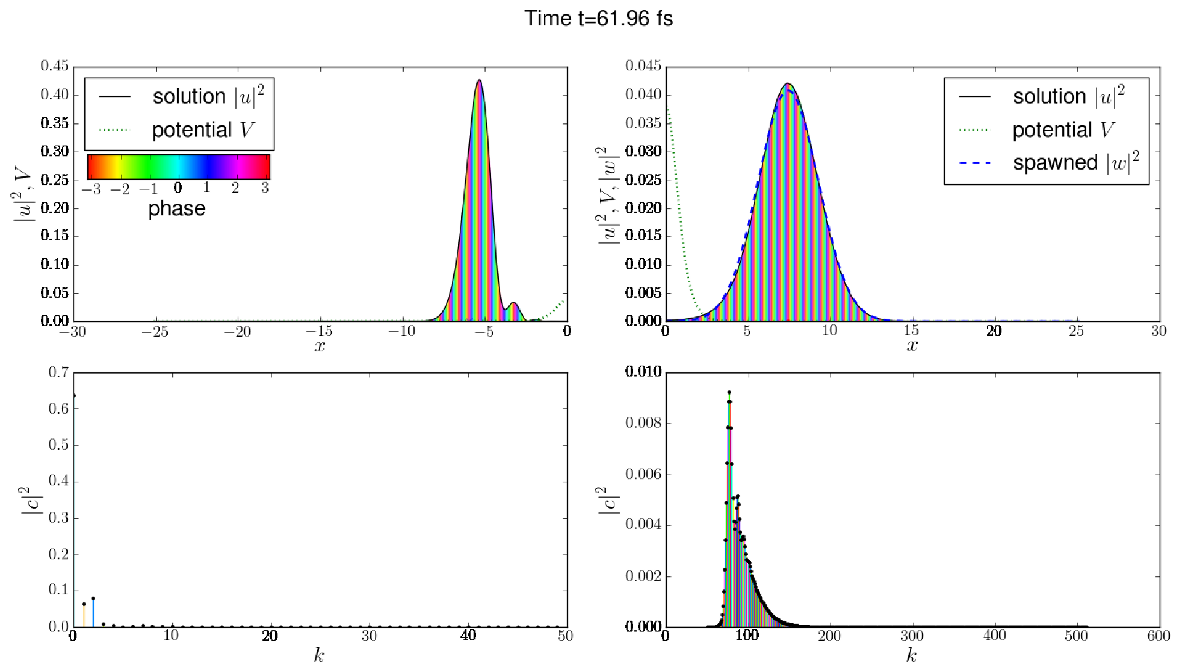
\includegraphics{./fig/spawned.png}
  \end{figure}
  \tiny{{taken from \cite{GHJ10a}}}
\end{frame}


\section{Future work}


\begin{frame}{Current research}
  \begin{itemize}
    \item Spawning in the \emph{non-adiabatic} case
  \end{itemize}
  \begin{figure}
    \centering
    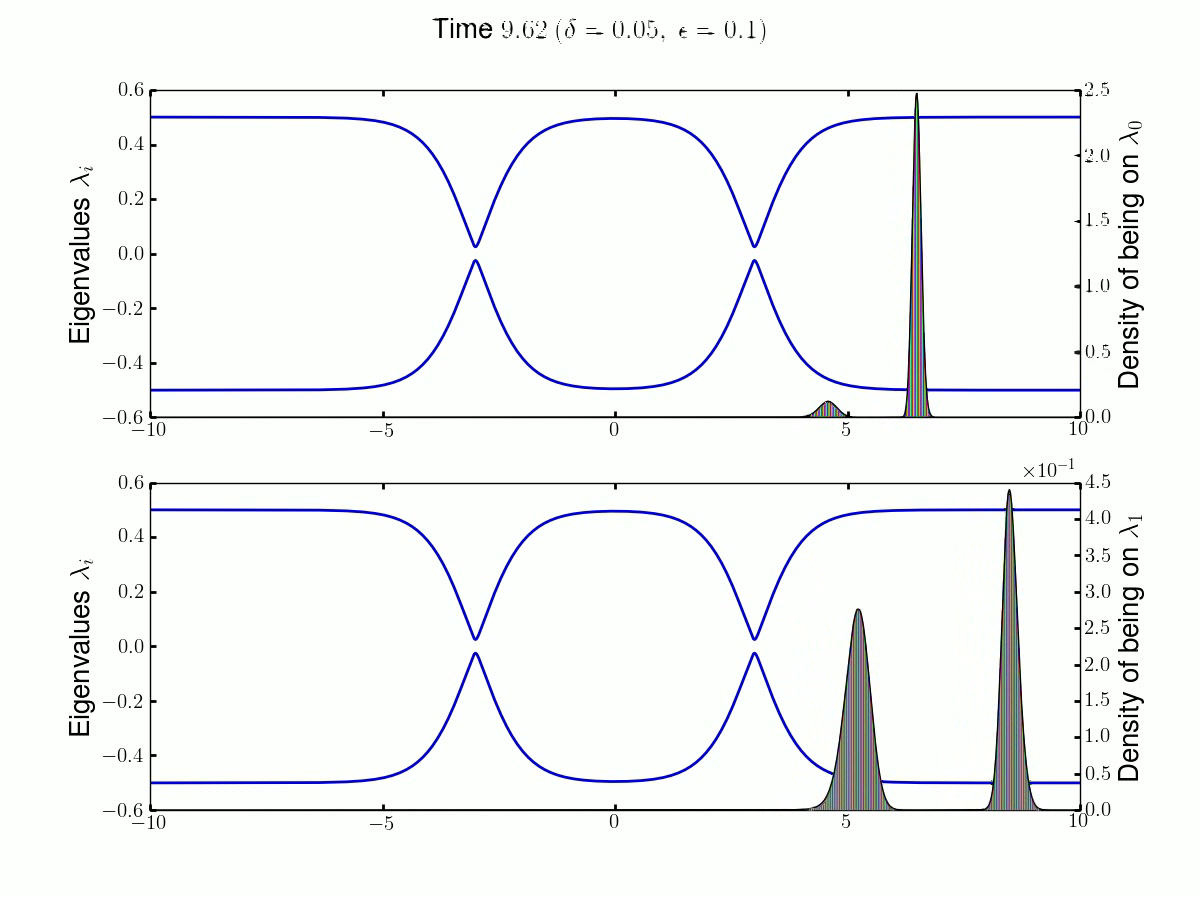
\includegraphics[scale=0.2]{./fig/nonadiabatic.png}
  \end{figure}
\end{frame}


\section{End}


\begin{frame}{Thanks for your attention}
  \bibliographystyle{siam}
  \bibliography{gradinaru}
\end{frame}

\end{document}
